\documentclass[10pt]{article}
\usepackage[margin=0.75in]{geometry}
\usepackage{microtype}
\usepackage{booktabs}
\usepackage{graphicx}
\usepackage{hyperref}
\usepackage{url}
\usepackage{enumitem}
\usepackage{titlesec}
\setlist{nosep}
% Tighten section spacing
\titlespacing*{\section}{0pt}{0.6ex}{0.3ex}
\titlespacing*{\paragraph}{0pt}{0.4ex}{0.5em}
\setlength{\parskip}{0.15ex}
\setlength{\abovecaptionskip}{2pt}
\setlength{\belowcaptionskip}{0pt}
\setlength{\textfloatsep}{4pt}
\setlength{\intextsep}{4pt}
\hypersetup{colorlinks=true,linkcolor=blue,citecolor=blue,urlcolor=blue}

\title{\vspace{-2.5em}\large Fine-Grained Classification of arXiv CS Abstracts:
A Linear-Probe Study Across Six Overlapping Sub-fields}
\author{\small Tian -- Uppsala University, NLP coursework}
\date{\vspace{-2ex}}

\begin{document}
\maketitle
\vspace{-3.5em}

\paragraph{Artefacts.}
\href{https://huggingface.co/datasets/Tiansve/arxiv-cs-subfield}{Dataset} ~|~
\href{https://huggingface.co/Tiansve/arxiv-subfield-linear-probe}{Model} ~|~
\href{https://huggingface.co/spaces/Tiansve/arxiv-subfield-demo}{Live demo (Gradio Space)}.

\section{Introduction}
arXiv lets a paper carry multiple categories, but exposes only one
\texttt{primary\_category}. I treat sub-field assignment as a single-label
classification problem over six categories
(\texttt{cs.CL}, \texttt{cs.LG}, \texttt{cs.CV}, \texttt{cs.IR}, \texttt{cs.AI},
\texttt{stat.ML}) that are well known to overlap in practice -- a paper on
transformer architectures could plausibly sit in three of them. The simplification
is therefore lossy by construction, which makes the task genuinely hard and
provides a natural error-analysis story rather than the toy
``physics-vs-biology'' setting often used as a baseline.

\section{Dataset}
I pulled metadata from the arXiv API~\cite{arxivapi} using the
\texttt{arxiv} v4 Python client with a 3.5\,s request delay. For each target
category, only papers whose \texttt{primary\_category} \emph{equals} the queried
category were retained, so the label is unambiguous. After deduplication, a
minimum-length filter (50 words of abstract), and balancing to the size of the
smallest class (\texttt{cs.AI}, 686 papers after filtering), I obtained
\textbf{4{,}116} rows across six classes. The data was split 80/10/10 train/val/test
in a stratified manner with \texttt{random\_state=42}, yielding sizes of 3{,}292 /
412 / 412. I deliberately kept LaTeX markup in abstracts as-is: modern
embedders have seen it, and stripping it loses information. The dataset is
published on the Hugging Face Hub with a full dataset card.

\section{Methods}
The task input is \texttt{title + ``. '' + abstract}; the label is a
human-readable mapping of \texttt{primary\_category}. I compared one
non-embedding baseline against five embedding-based configurations:
\begin{itemize}
\item \textbf{tfidf\_logreg} -- TF-IDF (10{,}000 features, 1--2 grams, sub-linear
  TF) plus logistic regression. This is the ``do embeddings help?'' baseline.
\item \textbf{mpnet\_\{logreg,linsvm,mlp\}} -- features from
  \texttt{all-mpnet-base-v2}~\cite{song2020mpnet,reimers2019sbert} fed to
  logistic regression, calibrated linear SVM, and an MLP$(256,128)$ respectively.
\item \textbf{minilm\_logreg} -- a smaller and faster
  \texttt{all-MiniLM-L6-v2}~\cite{wang2020minilm} feature space.
\item \textbf{e5\_logreg} -- \texttt{intfloat/e5-base-v2}~\cite{wang2022e5},
  with the model-card-recommended ``passage:'' prefix.
\end{itemize}
Embeddings were L2-normalised and cached to disk. LogReg's regularisation
$C\in\{0.1,1,10\}$ was tuned on validation; MLP and SVM used defaults. All
training and scoring used scikit-learn~\cite{pedregosa2011sklearn}.

\section{Results}
Selection was by validation macro-F1; test metrics are reported only for the
final comparison.

\begin{table}[h!]
\centering
\footnotesize
\begin{tabular}{lcccc}
\toprule
config & val macro-F1 & test acc.\ & test macro-F1 & test weighted-F1 \\
\midrule
mpnet\_logreg  & \textbf{0.7581} & 0.7136 & 0.7112 & 0.7116 \\
tfidf\_logreg  & 0.7499 & \textbf{0.7403} & \textbf{0.7390} & \textbf{0.7394} \\
mpnet\_linsvm  & 0.7460 & 0.7233 & 0.7200 & 0.7204 \\
mpnet\_mlp     & 0.7444 & 0.7282 & 0.7252 & 0.7256 \\
minilm\_logreg & 0.7356 & 0.7160 & 0.7124 & 0.7125 \\
e5\_logreg     & 0.7179 & 0.7063 & 0.7058 & 0.7060 \\
\bottomrule
\end{tabular}
\end{table}

\noindent The story is more interesting than ``embeddings win''.
\texttt{mpnet\_logreg} edges every other model on validation by $\leq 0.025$
macro-F1, but on test the TF-IDF baseline overtakes all five embedding
configurations. I attribute this to (i) the modest dataset size (412 test
examples spread over six classes makes individual class scores swing easily),
and (ii) arXiv abstracts being rich in field-specific vocabulary that TF-IDF
already captures well. The honest takeaway is that on this particular slice,
the embedding advantage is within noise -- a useful pedagogical result for
the report rather than a failure.

The per-class report for the winning \texttt{mpnet\_logreg} on test shows the
expected pattern (Fig.~\ref{fig:cm}): \texttt{ir\_retrieval} and
\texttt{stat\_ml} score above 0.80 F1 because their vocabulary is distinctive;
the confusable trio \texttt{cs.AI}, \texttt{cs.CL}, \texttt{cs.LG} sits at
0.58--0.65. The largest off-diagonal mass is between \texttt{ai\_general} and
\texttt{lg\_ml}, which is the exact qualitative behaviour the introduction
predicted.

\begin{figure}[h!]
\centering
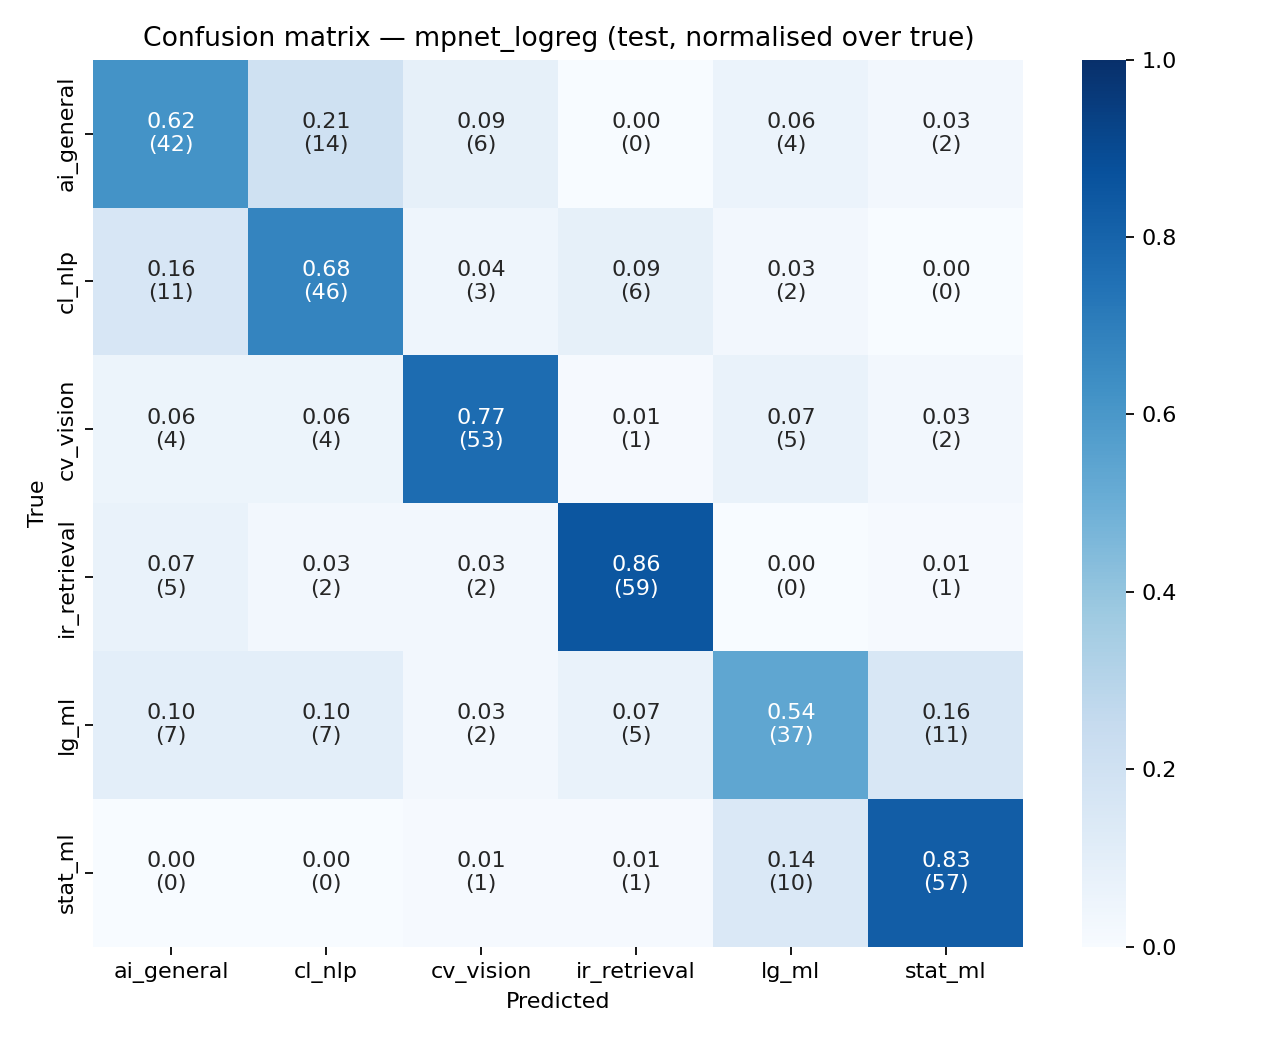
\includegraphics[width=0.50\linewidth]{../results/confusion_matrix.png}
\caption{\footnotesize Test-set confusion matrix for \texttt{mpnet\_logreg},
normalised over true labels (counts in parentheses).}
\label{fig:cm}
\end{figure}

\section{Reflection on Working with AI Tools}
This project was scaffolded with Claude Code (Anthropic's command-line coding
agent). The agent accelerated the boilerplate-heavy steps -- writing
\texttt{fetch\_arxiv.py}, the embedding cache layer, the upload scripts, and
the Gradio app skeleton -- by an estimated 3--4$\times$ relative to writing
them from scratch.

A concrete case where the AI was wrong and had to be corrected: when
\texttt{embed.py} first crashed with
\verb|OSError: [WinError 1114]| from \texttt{torch}, the agent's initial
hypothesis was a missing Visual C++ runtime. A diagnostic one-liner
(\texttt{python -c "import torch; from sentence\_transformers import ..."})
showed that torch \emph{did} load when imported in isolation. The real cause
was an MKL/OpenMP DLL clash between the conda-installed numpy and the
pip-installed torch 2.12+cpu: importing numpy first poisoned the symbol
table for torch's bundled MKL. The fix was to import torch \emph{before}
numpy in the entry-point scripts and set
\texttt{KMP\_DUPLICATE\_LIB\_OK=TRUE}. This was missed by the agent on first
attempt; only the empirical evidence from running both imports separately
revealed the ordering dependency. The lesson is that fast-moving Windows
DLL-loading issues are exactly the kind of environmental detail that an LLM
agent can speak confidently about while being wrong -- the cheap diagnostic
test was what caught it.

A second smaller case: the agent picked \texttt{python\_version: "3.11"}
late, after a first Space build failed because the default HF runtime had
moved to Python 3.13 (which drops \texttt{audioop}, breaking Gradio's
\texttt{pydub} dep). Pinning the runtime should have been in the original
plan; I only added it reactively.

\section{Conclusion and Limitations}
A frozen-embedding linear probe achieves macro-F1 $\approx 0.71$ on a
balanced 6-class arXiv sub-field classifier, with a TF-IDF baseline that is
indistinguishable from -- and on test slightly better than -- five different
embedding pipelines. Limitations: (i)~the single-label simplification of a
multi-label problem, (ii)~no temporal generalisation test (train, val, and
test all come from the same 2023--2025 window), and (iii)~$\sim 688$ papers
per class is small enough that test-set fluctuations dominate the model
ranking. A natural extension is to recast the task as multi-label using all
arXiv categories per paper, where the embedding advantage may reassert
itself.

\bibliographystyle{plain}
\bibliography{refs}

\end{document}
